\documentclass[fleqn,12pt,openany]{book}

% These two need to be set before including scirun style package
\title{SCIRun User Guide}
\author{SCIRun Development Team}

% INCLUDE SCI STYLE DOCUMENT
\usepackage{scirun}

\begin{document}

%% starting from SCIRun Doc wiki
%% http://software.sci.utah.edu/SCIRunDocs/index.php/CIBC:Documentation:SCIRun:Tutorial:BioPSE


% CREATE TITLE PAGE --------------------------------------------------
\maketitle

% CHAPTERS ---------------------------------------------------------------

\chapter{SCIRun Introduction}\label{intro}

\begin{introduction}
SCIRun is a \emph{modular dataflow programming} Problem Solving Environment (PSE).
SCIRun has a set of Modules that perform specific functions on a data stream.
Each module reads data from its input ports, calculates the data, and sends new data from output ports.
\end{introduction}

In SCIRun, a module is represented by a rectangular box on the Network Editor canvas.
Data flowing between modules is represented by pipes connecting the modules.
A group of connected modules is called a Dataflow Network, or net (see figure \ref{sample_network}).
An infinite number of nets can be created, each solving a separate problem.
Chapter \ref{intro} of this tutorial demonstrates the use of SCIRun to visualize
a tetrahedral mesh.

This chapter demonstrates the construction of a network comprised of three
standard modules: ReadField, ShowField, and ViewScene.
This chapter also instructs the user on reading Field data from a file, setting
rendering properties for the nodes, edges, and faces (the nodes are rendered as
blue spheres), and rendering geometry to the screen in an interactive ViewWindow.

\begin{figure}[H]\label{sample_network}
\begin{centering}
\scalebox{0.5}{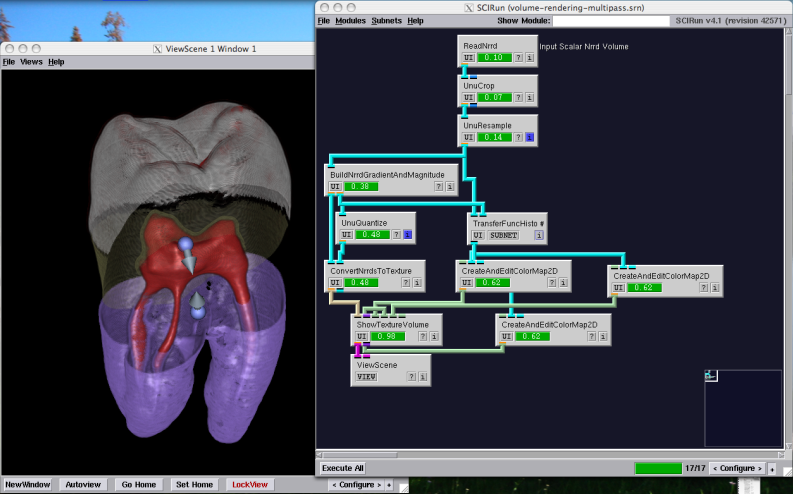
\includegraphics{UserGuide_figures/sample_network.png}}
\caption{SCIRun Dataflow Network}
\end{centering}
\end{figure}

\section{Starting SCIRun}
\subsection{SCIRun usage}
Use the \textbf{--help} flag for SCIRun usage and a full list of command line flags.

\begin{verbatim}
Usage: scirun [args] [net_file] [session_file]
    [-]-d[atadir]            : scirun data directory
    [-]-r[egression]         : regression test a network
    [-]-R[egressionimagedir] : output directory for regression tests
    [-]-s[erver] [PORT]      : start a TCL server on port number PORT
    [-]-e[xecute]            : executes the given network on startup
    [-]-E[xecute]            : executes the given network on startup and
                               quits when done
    [-]-c[onvert]            : converts a .net to a .srn network and exits
    [-]-v[ersion]            : prints out version information
    [-]-h[elp]               : prints usage information
    [-]-p[ort] [PORT]        : start remote services port on port number PORT
    [-]-l[ogfile] file       : add output messages to a logfile
    [-]-t[imeout] N          : kill scirun after N seconds
    [-]-I[mage] file         : Save resulting images in file
    [--nosplash]             : disable the splash screen
    net_file                 : SCIRun Network Input File
    session_file             : PowerApp Session File
\end{verbatim}

\subsection{Preparation for Unix, Mac, Linux, etc.}

Preparations must be made before starting SCIRun and its PowerApps.
Commands below are typed in a terminal emulation application (e.g. xterm).
See SCIRun's initialization file \emph{\$HOME/.scirunrc} for additional information.
Change directory to SCIRun's build directory and start SCIRun from the command line:
  
\begin{verbatim}
cd SCIRun/bin
./scirun [--execute] [network_file]
\end{verbatim}

The \textbf{scirun} command may take the name of a SCIRun network file (network files have a \textbf{.srn} extension) for SCIRun to load.
The \textbf{--execute} flag tells SCIRun to execute the network after it is loaded.
Network files are discussed in a later section.

\begin{centering}
\textbf{\textsf{Do not start SCIRun in the background, i.e. do not type: scirun \&.}}
\end{centering}

\subsubsection{Mac OS X 10.4}

Run SCIRun in the X11 Terminal.
If the binary package has been installed, the SCIRun application can be launched from Finder.

\begin{figure}[H]
\begin{centering}
\scalebox{0.5}{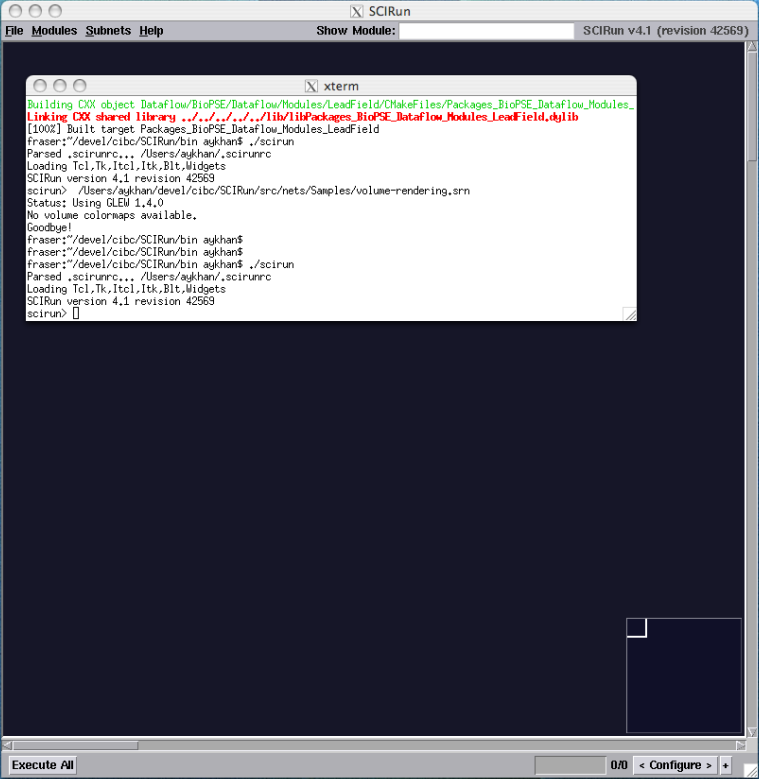
\includegraphics{UserGuide_figures/osx_10_4_startup.png}}
\caption{SCIRun on OS X 10.4}
\end{centering}
\end{figure}

\subsection{Preparation for Windows}

In Windows, SCIRun can be stared from Explorer, or launched from a
``Windows Command Prompt'' (cmd.exe).
Alternatively, you can start it up by browsing My Computer or Windows Explorer
to the directory that contains scirun.exe and double-clicking on it.
%% User application data folder location obtained from registry key
%% HKEY_CURRENT_USER\Volatile Environment\APPDATA
%%
%% Typical values are
%% Vista: c:\Users\<user account name>\AppData\Roaming\SCIRun
%% XP: c:\Documents and Settings\<user account name>\Application Data\SCIRun
The SCIRun initialization file \emph{.scirunrc} can be found in the user applicaton data folder.
Command line flags are the same as for Unix platforms.

\begin{verbatim}
cd ``c:\Program Files\SCIRun 4.0\bin''
scirun.exe [--execute] [network_file]
\end{verbatim}

If you install the Windows binary version of SCIRun or associate .srn files with SCIRun, you can also double-click on any scirun
network file (.srn) and it will run SCIRun with that network file.
To associate srn files with SCIRun, do the following:

\begin{enumerate}
\item Open a Windows Explorer window, click the Tools menu and select Options
\item Click the File Types tab, and select New
\item In the Dialog that appears, type \textbf{srn} and click OK
\item In the Details for SRN extension frame, click \textbf{Change} and navigate to scirun.exe
\end{enumerate}

\subsection{Post startup}

If the name of a network file is not provided, SCIRun starts with an empty window as shown below.

\begin{figure}[ht]
\begin{centering}
\scalebox{0.5}{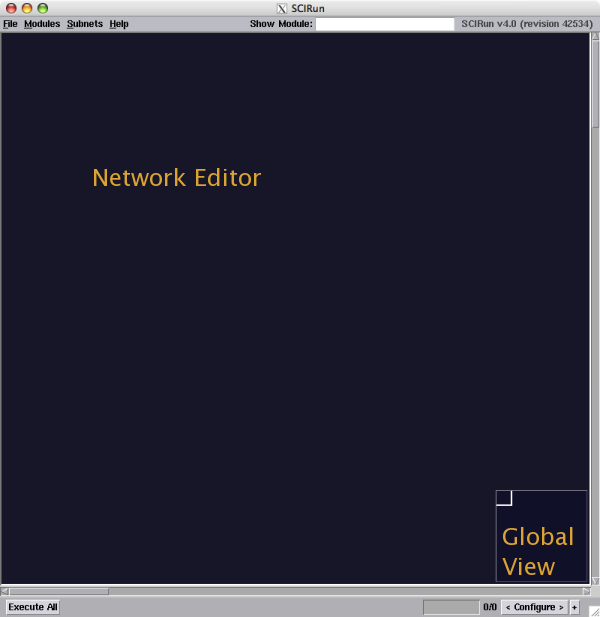
\includegraphics{UserGuide_figures/blankSCIRun.png}}
\caption{SCIRun initial NetworkEditor window}
\end{centering}
\end{figure}

SCIRun may encounter errors during start up.
%% TODO: show image
Errors, warnings, and other messages are displayed in SCIRun's log console.
Errors should be reported to the SCIRun development team at
\href{mailto:scirun-develop@sci.utah.edu}{scirun-develop@sci.utah.edu}.
Developers with SCI or SCI collaborator accounts can report bugs and request features through the
tracker on the \href{https://gforge.sci.utah.edu/gf/project/cibc/tracker}{SCI GForge portal}. 

\subsubsection{Remote Display}
Normally, SCIRun's main window is displayed on a console that is part of the computer on which SCIRun runs.
It is possible, however, to display SCIRun on a remote console.
In the discussion that follows, the term local refers to the machine running SCIRun and the term remote refers to the machine displaying SCIRun.

\begin{quote}
\begin{centering}
\emph{Advanced GL remote rendering is problematic.}
\end{centering}
\end{quote}

SCIRun is compiled against the GL driver on the local machine, but when displayed remotely, uses the remote machine's GL driver.
Many times the local and remote drivers are not compatible and will result in SCIRun crashing.
For this reason, if possible, try not to run SCIRun in this manner.

To display SCIRun remotely, the value of the \textbf{DISPLAY} environment variable must be set correctly on the local machine.
Also, the local machine must be allowed to send display commands to the remote machine.

Normally, the remote machine makes a connection to the local machine via the ssh command.
In this case, ssh sets the value of DISPLAY in such a way that the local machine has permission to send display commands to the remote machine.
However, ssh connections result in poor display performance because of encryption activity on the connection.

To increase performance, the value of DISPLAY is set after establishing the ssh connection.

For a sh-style shell:

\begin{verbatim}
   export DISPLAY=remote-machine-name:0.0
\end{verbatim}

For a csh-style shell:

\begin{verbatim}
   setenv DISPLAY remote-machine-name:0.0
\end{verbatim}

Note that this technique defeats the encryption protection on the connection.

After overriding the value of DISPLAY set by ssh, the local machine will lack permission to send display commands to the remote machine.
Use the xhost command on the remote machine to give permission to the local machine:

\begin{verbatim}
   xhost +local-machine-name
\end{verbatim}

\subsection{Anatomy of the Main Window}
The SCIRun main window consists of the Menu Bar, the Global View frame, the Message frame, and the Net Edit frame.

\begin{customdesc}
\item[Menu Bar]
The menu bar is used to load networks, save networks, quit SCIRun, create network modules, and perform other tasks.
The menu bar consists of the following menu items:
  \begin{customdesc}
  \item[File]
  The File menu contains the following items:
    \begin{customdesc}
    \item[Load]
    Loads a network from a file
    \item[Insert]
    Adds a network to the NetEdit frame without overlap.
    \item[Save]
    Saves a network to a file
    \item[Save As...]
    Saves a network to a new file
    \item[Clear Network]
    Removes all modules and connections from the NetEdit frame
    \item[Select All]
    Selects all modules.
    \item[Execute All]
    Executes all modules.
    \item[Create Module Skeleton...]
    Contains the Create Module Skeleton option which guides a user through the creation of a basic module.
    \item[Quit]
    Quits SCIRun.
    Pressing key combination Control-q also quits.
    \emph{Do not press Control-c to exit SCIRun: doing this will drop SCIRun into a debugger.}
    \end{customdesc}
  \end{customdesc}
\item[Modules]
This menu is composed of sub-menus.
Each sub-menu corresponds to a category within the SCIRun package database.
A category is a group of related modules.
Each menu item in a category sub-menu creates a specific module and places it in the NetEdit frame.
The NetEdit frame pop-up menu also provides access to the SCIRun and BioPSE (and possibly other) package menus.
Activate the NetEdit frame pop-up menu by clicking the right mouse button (Btn3).
  \begin{customdesc}
  \item[SCIRun]
  The SCIRun menu is used to create modules (from the SCIRun package) for use in the Net Edit frame.
  \item[BioPSE]
  The BioPSE menu creates modules (from the BioPSEpackage) for use in the NetEdit frame.
  It consists of category sub-menus and module menu items.
  \item[Other Package Menus]
  There may be other package menus if other packages have been installed.
  They also have category sub-menus and module menu items.
  \end{customdesc}
\item[Subnets]
%% TODO: definition needed
\item[Global View Frame]
The Global View Frame is located in the lower right corner of the main window.
It is used to navigate complex networks.
\item[NetEdit Frame]
The NetEdit Frame occupies the main window.
It is used to build and execute networks.
\item[Show Module]
%% TODO: definition needed
\item[Configure Frame]
%% TODO: update to describe dockable frame
This dockable frame contains three tabs.
Toggle expanding the Configure frame by pressing the \textbf{Configure} button.
Toggle the frame's docking mode by pressing the button to the right of the Configure button.
  \begin{customdesc}
  \item[Network Editor]
\begin{figure}[H]\label{net_ed_options}
\begin{centering}
\scalebox{0.5}{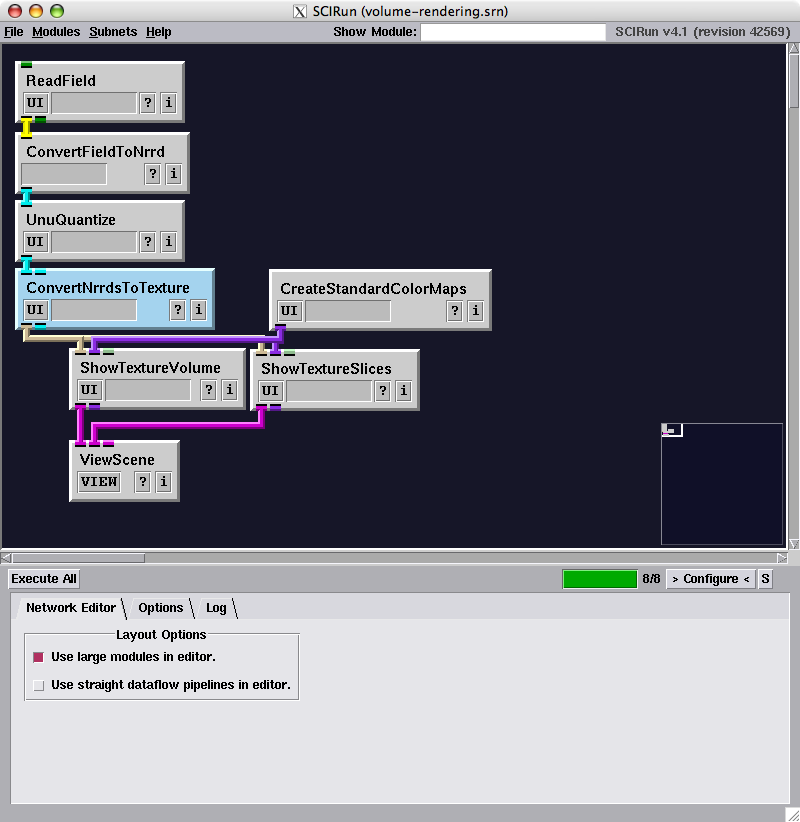
\includegraphics{UserGuide_figures/net_ed_options.png}}
\caption{SCIRun NetworkEditor configure options}
\end{centering}
\end{figure}
  \item[Options]
\begin{figure}[H]\label{misc_options}
\begin{centering}
\scalebox{0.5}{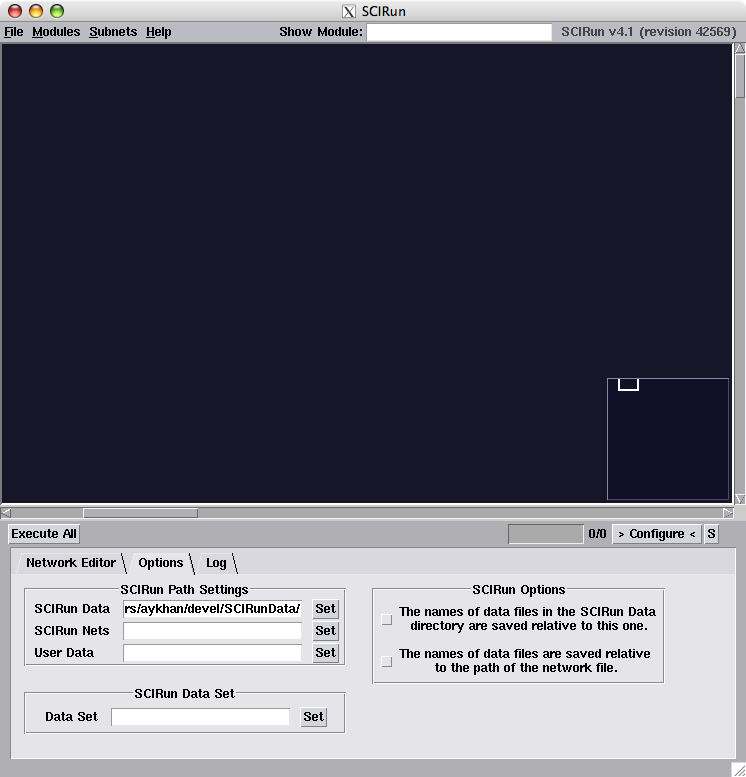
\includegraphics{UserGuide_figures/misc_options.png}}
\caption{SCIRun configure options}
\end{centering}
\end{figure}
  \item[Log]
Messages during program startup are displayed in the Message frame.
The Message frame reports errors, warnings, and important information.
Errors on startup may mean SCIRun has been installed incorrectly or has been installed from a buggy distribution; please report these errors.

\begin{figure}[H]\label{log_window}
\begin{centering}
\scalebox{0.5}{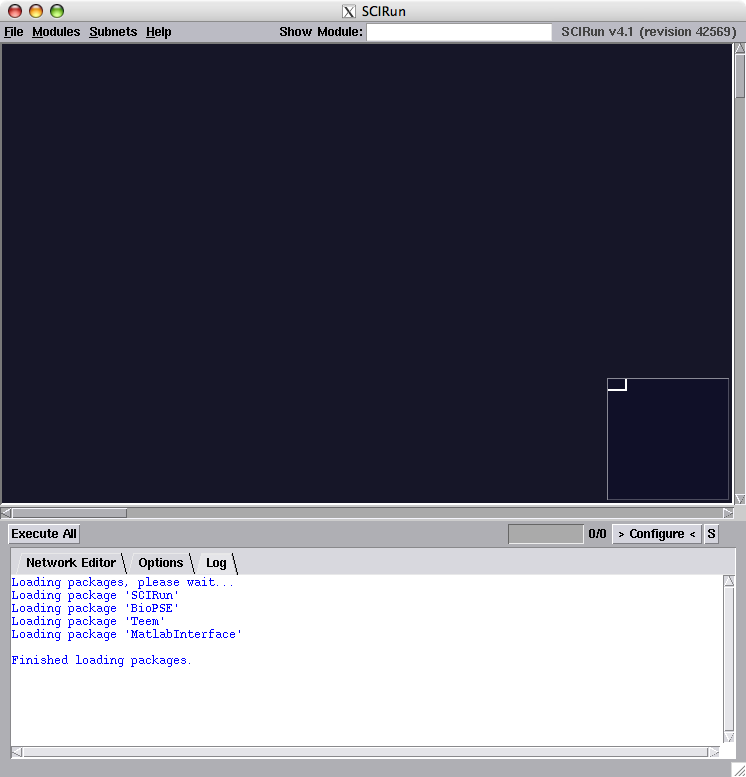
\includegraphics{UserGuide_figures/log_window.png}}
\caption{SCIRun log messages}
\end{centering}
\end{figure}
  \end{customdesc}
\end{customdesc}

\subsection{The Terminal Window}

After starting, SCIRun runs a shell-like application in the terminal window called the SCIRun shell.
The SCIRun shell displays the prompt \texttt{scirun>}.
This program is a modified Tool Command Language (TCL) shell program.
It is possible to type TCL'ish SCIRun commands at the prompt.
A later section describes use of the SCIRun shell.

\subsubsection{SCIRun's Environment}
SCIRun responds to a number of variables to alter its default behavior.
They can be in two places: the .scirunrc file, or in environment variables.

When started by a user the first time, SCIRun creates a default version of .scirunrc in the user's home directory (for unix-based environments) or in the directory that you compiled or installed scirun.exe in (for windows).
Users may modify their default .scirunrc file.

SCIRun then processes the .scirunrc file on each subsequent startup.
The .scirunrc file contains assignments to environment variables that affect SCIRun's behavior.
Lines beginning with '\#' are ignored.

Users may also set SCIRun related environment variables in their shell.
Values of variables set in the shell override values set in .scirunrc.

See the content of .scirunrc for a complete list of SCIRun related environment variables.
The following is a partial list of variables understood by SCIRun.

\subsubsection{The Initialization File}

The contents of \textbf{.scirunrc} look typically like:

\begin{verbatim}
#
#  For more information, please see: http://software.sci.utah.edu
# 
#  The MIT License
# 
#  Copyright (c) 2009 Scientific Computing and Imaging Institute,
#  University of Utah.
# 
#  
#  Permission is hereby granted, free of charge, to any person obtaining a
#  copy of this software and associated documentation files (the "Software"),
#  to deal in the Software without restriction, including without limitation
#  the rights to use, copy, modify, merge, publish, distribute, sublicense,
#  and/or sell copies of the Software, and to permit persons to whom the
#  Software is furnished to do so, subject to the following conditions:
# 
#  The above copyright notice and this permission notice shall be included
#  in all copies or substantial portions of the Software.
# 
#  THE SOFTWARE IS PROVIDED "AS IS", WITHOUT WARRANTY OF ANY KIND, EXPRESS
#  OR IMPLIED, INCLUDING BUT NOT LIMITED TO THE WARRANTIES OF MERCHANTABILITY,
#  FITNESS FOR A PARTICULAR PURPOSE AND NONINFRINGEMENT. IN NO EVENT SHALL
#  THE AUTHORS OR COPYRIGHT HOLDERS BE LIABLE FOR ANY CLAIM, DAMAGES OR OTHER
#  LIABILITY, WHETHER IN AN ACTION OF CONTRACT, TORT OR OTHERWISE, ARISING
#  FROM, OUT OF OR IN CONNECTION WITH THE SOFTWARE OR THE USE OR OTHER
#  DEALINGS IN THE SOFTWARE.
#

#
# Sample .scirunrc file.
#
# This file is copied from the SCIRun src tree file:
#   ./SCIRun/src/scirunrc
#
# Lines beginning with '#' are commented out.
#
# All variables in this file have been commented out or set
# to their default values.
#
# This file contains a list of environment variables that can be either set
# in your shell or here. If you set these variables in your shell, they will 
# override the values in this file.
#
# All variable declarations must use the syntax:
#    Environment_Variable_Name = Value
#
# Boolean variable declarations use this syntax:
#    Environment_Variable_Name = <true,1,on,yes|false,0,off,no>
#

#####################################
### ENVIRONMENT VARIABLES SECTION ###
#####################################

# REMEMBER, if these variables are set in your shell environment, they will
# override the valuse in this file.

### SCIRUN_ACCEPT_LICENSE
# Records whether license was accepted
# SCIRUN_ACCEPT_LICENSE = true

### SCIRUN_LOAD_PACKAGE = [comma-seperated list]
#   The format of SCIRUN_LOAD_PACKAGE is a comma seperated list of
#   package names.  This list specifies the package libraries to load
#   when SCIRun is first brought up.
# SCIRUN_LOAD_PACKAGE = BioPSE,Uintah,Teem


### SCIRUN_SHOW_HIDDEN_MODULES = [boolean]
#   Show modules that have been set to be hidden. These hidden modules include
#   obsolete or unfinished modules. Use extra care when using these modules
#   as they may be deleted in a future version or may cause scirun to crash
# SCIRUN_SHOW_HIDDEN_MODULES = true

### SCIRUN_DATA = [path]
#   Directory location that 'Reader' modules will default to.
# SCIRUN_DATA = /usr/sci/data/SCIRunData

### SCIRUN_DATASET = [name]
#   Name of data set in SCIRUN_DATA to default to.
# SCIRUN_DATASET = sphere


### SCIRUN_NET_SUBSTITUTE_DATADIR = [boolean]
#   If true, module filename variables will be automatically substituted for
#   'SCIRUN_DATADIR' and 'SCIRUN_DATASET' in saved .net files.
# SCIRUN_NET_SUBSTITUTE_DATADIR = false

### SCIRUN_NET_RELATIVE_FILENAMES = [boolean]
#   If true, SCIRun will save all filenames relative to the location of the 
#   network file in the .srn files.
# SCIRUN_NET_RELATIVE_FILENAMES = true


### SCIRUN_MYDATA_DIR = [path]
#   Directory, or list of directories separated by colons, 
#   that data 'Reader' and 'Writer' modules will list as
#   optional paths in the directories drop down menu.
# SCIRUN_MYDATA_DIR = $HOME/data:/scratch/data

### SCIRUN_NET_DIR = [path]
#   Directory, or list of directories separated by colons, 
#   that the network editor will list as
#   optional paths in the directories drop down menu.
# SCIRUN_NET_DIR = [path]

### SCIRUN_TMP_DIR = [path]
#   Directory for writting temporary files - must be world read/writeable
# SCIRUN_TMP_DIR = /tmp

### SCIRUN_SERV_TMP_DIR = [path]
#   Directory for writting temporary files - must be world read/writeable
#   This is one is used by the external application interface. Both scirun
#   and scirunremote use this one to exchange files.
# SCIRUN_SERV_TMP_DIR = /tmp

### SCIRUN_CONFIRM_OVERWRITE = [boolean]
#   If false, SCIRun writer will not prompt the user before overwriting a file
# SCIRUN_CONFIRM_OVERWRITE = true


### SCIRUN_INSERT_NET_COPYRIGHT = [boolean]
#   If true, adds SCI copyright to any SCI .net files that are created.
# SCIRUN_INSERT_NET_COPYRIGHT = false

### SCIRUN_NOSPLASH = [boolean]
#   If true, SCIRun will not display the splash screen at startup.
# SCIRUN_NOSPLASH = false


### SCIRUN_HIDE_PROGRESS = [boolean]
#   If true, SCIRun will not display progress bars during startup and loading
# SCIRUN_HIDE_PROGRESS = false


### SCIRUN_FAST_QUIT = [boolean]
#   If true, SCIRun will not ask the user to save a network before quitting
# SCIRUN_FAST_QUIT = false

### SCI_REGRESSION_TESTING = [boolean]
#   If True, regression testing mode will turn on.  Execution starts after a
#   network is loaded and SCIRun will exit immediately after creating an image.
# SCI_REGRESSION_TESTING = false


### SCIRUN_REGRESSION_TESTING_TIMEOUT = [integer]
#   If set, and if SCI_REGRESSION_TESTING is True, SCIRun will automatically
#   kill itself after specified seconds.
# SCI_REGRESSION_TESTING_TIMEOUT = 300


### THREAD_NO_CATCH_SIGNALS = [boolean]
#   Turns off the SCI Signal handlers.
# THREAD_NO_CATCH_SIGNALS = true


### SCIRUN_DRAWARRAYS_DISABLE = [boolean]
#   Turns off use of glDrawArrays.  This should be set to true if you wish
#   to avoid drawing artifacts on _ATI_ Radeon cards under Linux or to fix
#   cross-platform remote display problems.
# SCIRUN_DRAWARRAYS_DISABLE = false


### SCIRUN_MPEG_LICENSE_ACCEPT = [boolean]
#   License information describing the mpeg_encode software can be found
#   in SCIRun's Thirdparty directory, in the mpeg_encode/README file:
#   This software is freely distributed.  That means, you may use it
#   for any non-commercial purpose.  However, patents are held by
#   several companies on various aspects of the MPEG video standard.  
#   Companies or individuals who want to develop commercial products 
#   that include this code must acquire licenses from these companies.  
#   For information on licensing, see Appendix F in the standard.
#   For more information, please see the mpeg_encode README file.
#   If you are allowed to use the MPEG functionality based on the above
#   license, you may
#   enable MPEG movie recording in SCIRun (accessible via the SCIRun
#   Viewer's "File->Record Movie" menu) by setting the value of
#   SCIRUN_MPEG_LICENSE_ACCEPT to "true".
# SCIRUN_MPEG_LICENSE_ACCEPT = false

### SCIRUN_USE_DEFAULT_SETTINGS = [boolean]
#   Force the sizes for ShowField to calculate defaults when loading a new 
#   Field.  Also Forces the Viewer to autoview whenever a new netork is
#   loaded.
#SCIRUN_USE_DEFAULT_SETTINGS = true

### DISABLE_MATLAB_PROCESS
# Disable forking of SCIRun on start of SCIRun to support Matlab running in
# separate process
# DISABLE_MATLAB_PROCESS = true

############################
# GUI PREFERENCES SECTION ##
############################

### SCIRUN_GUI_UseGuiFetch = [boolean]
#   Allows the user to tell a module to fetch the GUI from wherever it
#   happens to be on the screen and bring it to the mouse, and then
#   return it to its previous location.
SCIRUN_GUI_UseGuiFetch = on

### SCIRUN_GUI_MoveGuiToMouse = [boolean] 
#   Makes GUIs appear near the mouse on GUI creation. 
SCIRUN_GUI_MoveGuiToMouse = on


### SCIRUN_STRAIGHT_CONNECTIONS = [boolean]
#   Use straight lines to represent connections between modules in the
#   network editor.
# SCIRUN_STRAIGHT_CONNECTIONS = off

### SCIRUN_LARGE_MODULES = [boolean]
#   Use a large module layout instead of a smaller one
# SCIRUN_LARGE_MODULES = off


#################
# UNDOCUMENTED ##
#################
# LOGNAME
# USER
# SCI_DEBUG
\end{verbatim}

\section{SCIRun Data Variables}

For convenience, the SCIRUN\_DATA environment variable (and optionally SCIRUN\_DATASET) can be set before starting SCIRun.
Alternatively, use the \textbf{--datadir} flag when starting SCIRun.

%%See the SCIRun's Environment section of the User Guide for information on how to set up this and other environment variables.

\begin{customdesc}
\item[SCIRUN\_DATA]
Points to the location of the SCIRunData directory on the system.
Note: it is assumed the SCIRunData directory has already been downloaded
(this is a separate download from the SCIRun build).
\item[SCIRUN\_DATASET]
Indicates which dataset to load.
For example, in SCIRunData, SCIRUN\_DATASET can be aneurysm, sphere, utahtorso etc.
%% Corresponds to subdirectory in SCIRunData.
%% TODO: move specific tutorial examples.
%%Note: example networks built in this tutorial can run with a variety of data inputs: e.g. sphere, brain-EG, and utahtorso-lowres.
\item[SCIRUN\_DATAFILE]
\end{customdesc}
%%Set these environment variables to the following values (See Figures ??? (csh/tcsh) and ??? (bask,ksh,sh)):

%% TODO: move specific tutorial examples.
%%       Update to go with tutorial network?
%% If not, at least check these instructions to make sure they still work.
%%Set the SCIRUN\_DATASET variable to ``utahtorso-lowres''.

%%[[Image:1 2.gif]]  Figure 1.0: Set environment variables using C-style shell (csh, tcsh).
%%[[Image:1 2b.gif]]   Figure 1.1: Setup using a Borne-style shell (bash, ksh, sh).


\subsubsection{Setting environment variables}
For unix environments, environment variables may be set as shown above in the SCIRUN\_DATA section.

For windows environments, follow these directions:
Click the Start button, select Control Panel, and then System.
In the Advanced tab, click the Environment Variables button.
Select New and enter the name and value of the environment variable.
If it already exists, click on it and select Edit to modify it.

\chapter{SCIRun Networks}

\section{SCIRun Network Building Blocks}

%%Lets begin constructing the network pictured in '''Figure 1.3'''.
%%(Note: subsequent tutorial chapters expand on this network, adding more features and functionality.) This network loads a geometric mesh from a data file and renders it to the screen.

%%[[Image:Chap1Net.gif]]<br />'''Figure 1.3: SCIRun NetworkEditor after building the Chapter 1 network.'''

%% TODO: More info on old doc site.
%% TODO: BioPSE module and connection diagram

\subsection{Modules}\label{modules}

A module is a single-purpose unit that functions within a dataflow environment.
Modules have at least one input port for receiving data, located at the top of the module, or one output port for sending data, located at the bottom of the module.
%%(See </nowiki>'''Figure 1.4''')

For a more complete description of modules, consult the \href{http://software.sci.utah.edu/SCIRunDocs/index.php/CIBC:Documentation:SCIRun:UserGuide:Concepts#SCIRun_Modules.2C_Networks.2C_and_Sub-Networks}{SCIRun Modules, Networks, and Sub-Networks Section of the User Guide}.

All modules have an indicator that alerts the user to messages that exist in a module's log. Different colors represent different types of messages.
Gray means no message, blue represents a Remark, yellow a Warning, and red an Error.
To read messages, click the module's indicator button to open the log window.
%%<center>[[Image:FieldReaderIcon.gif]]<br />'''Figure 1.4: SCIRun Module Icon.'''

- module categories


\subsection{Connections}\label{connections}

Data is transfered from one module to another using dataflow connections,commonly refered to as \textbf{pipes}.
Each dataflow pipe transfers a specific datatype in SCIRun, denoted by a unique color.
Pipes run from the output \textbf{port} of one module to the input port(s) of one or more other modules.
Ports of the same color correspond to the same datatype and can be connected.
These colors are described in detail in the \href{http://software.sci.utah.edu/SCIRunDocs/index.php/CIBC:Documentation:SCIRun:UserGuide:Networks#Anatomy_of_a_Module}{Anatomy of a Module} Section of the User Guide.

%% TODO
%%\section{Building Dataflow Networks}
%%
%%- basics
%%
%%- how to connect modules (mouse functions)
%%
%%- UIs

\section{Loading Data}

Load data using reader or importer modules in the DataIO module category.
Supported file formats can be found in chapter \ref{sec:formats}.

%% TODO
%%\section{Network Example}

\chapter{SCIRun Objects}

\section{Mesh}

SCIRun meshes are classified as unstructured, structured, or regular.
A mesh consists of nodes and implicit or explicit node connectivity information.


Node locations and connectivities for unstructured meshes are specified explicitly.
Node locations are specified explicitly, and connectivities are known implicitly for structured meshes.
Node locations and connectivities are known implicitly for regular meshes.

A regular mesh is more constrained than structured and unstructured meshes.
Likewise, a structured mesh is more constrained that a unstructured mesh.
A more constrained mesh can be trivially converted to a less constrained mesh by explicitly enumerating implicit properties.
For instance, a LatVol mesh is converted to a StructHexVol by enumerating a LatVol mesh's node coordinates (connectivities are still implied).
Also, a LatVol mesh is converted to a HexVol mesh by enumerating a LatVol's node locations and connectivities.
Module ToStructured performs this type of conversion.

It is not meaningful to convert a less constrained mesh to a more constrained mesh.
It is possible, however, to sample an unstructured field at regular intervals to create a regular field.
For example, a HexVolField is interpolated onto a LatVol mesh using modules SampleLattice and DirectInterpolate.

\subsection{Unstructured Meshes}

\subsubsection{CurveMesh}
\begin{figure}[H]\label{curvemesh}
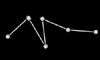
\includegraphics{UserGuide_figures/CurveMesh.png}
\caption{Curve Mesh}
\end{figure}

A curve mesh is a segmented curve.

\subsubsection{HexVolMesh}
\begin{figure}[H]\label{hexvolmesh}
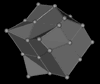
\includegraphics{UserGuide_figures/HexVol.png}
\caption{HexVol Mesh}
\end{figure}

A hex volume mesh is a subdivision of space into hexagonal elements.

\subsubsection{PointCloudMesh}
\begin{figure}[H]\label{pointcloudmesh}
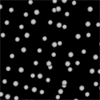
\includegraphics{UserGuide_figures/PointCloud.png}
\caption{Point Cloud Mesh}
\end{figure}

A point cloud  mesh is a set of unconnected points.

\subsubsection{PrismVolMesh}
\begin{figure}[H]\label{prismvolmesh}
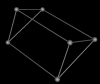
\includegraphics{UserGuide_figures/PrismVol.png}
\caption{PrismVol Mesh}
\end{figure}

A Prism Volume mesh  is a subdivision of space into prism elements.
Prism elements have five faces, two trangular faces connected by three quadrilateral faces. 

\subsubsection{QuadSurfMesh}
\begin{figure}[H]\label{quadsurfmesh}
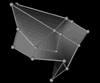
\includegraphics{UserGuide_figures/QuadSurf.png}
\caption{QuadSurf Mesh}
\end{figure}

A surface made of connected quadrilaterals.

\subsubsection{TetVolMesh}
\begin{figure}[H]\label{tetvolmesh}
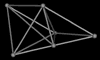
\includegraphics{UserGuide_figures/TetVol.png}
\caption{TetVol Mesh}
\end{figure}

A tet volume mesh is a subdivision of space into tetrahedral elements.

\subsubsection{TriSurfMesh}
\begin{figure}[H]\label{trisurfmesh}
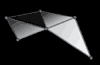
\includegraphics{UserGuide_figures/TriSurf.png}
\caption{TriSurf Mesh}
\end{figure}

A tri surface mesh is a surface made of connected triangles.

\subsection{Structured Meshes}

\subsubsection{StructCurveMesh}

\subsubsection{StructHexVolMesh}
\begin{figure}[H]\label{structhexvolmesh}
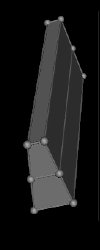
\includegraphics{UserGuide_figures/StructHexVol.png}
\caption{StructHexVol Mesh}
\end{figure}

A subdivision of space into structured hexagonal elements.

\subsubsection{StructQuadSurfMesh}
\begin{figure}[H]\label{structquadsurfmesh}
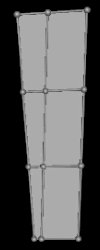
\includegraphics{UserGuide_figures/StructQuadSurf.png}
\caption{StructQuadSurf Mesh}
\end{figure}

A surface made of connected quadrilaterals on a structured grid.

\subsection{Regular Meshes}

\subsubsection{ImageMesh}
\begin{figure}[H]\label{imagemesh}
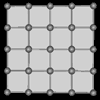
\includegraphics{UserGuide_figures/ImageField.png}
\caption{Image Mesh}
\end{figure}

An Image mesh is a regular 2D grid.
Note that an Image mesh is not used for image processing.

\subsubsection{LatVolMesh}
\begin{figure}[H]\label{latvolmesh}
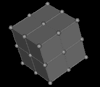
\includegraphics{UserGuide_figures/LatticeVol.png}
\caption{LatVol Mesh}
\end{figure}

A lattice volume mesh is a regular 3D grid.

\subsubsection{ScanlineMesh}
\begin{figure}[H]\label{scanlinemesh}

\includegraphics{UserGuide_figures/ScanlineField.png}
\caption{Scanline Mesh}
\end{figure}

A scanline mesh is a regularly segmented straight line (a regular 1D grid).

\section{Field}

A Field contains a geometric mesh, and a collection of data values mapped on to the mesh.
Data can be stored at the nodes, edges, faces, and/or cells of the mesh.
%%In this case, a tetrahedral mesh with voltages defined at the nodes of the mesh has been selected.

\section{Storing types in SCIRun Field}
%% see http://www.sci.utah.edu/SCIRunDocs/index.php/CIBC:Documentation:SCIRun:UserGuide:ImportExport

The dimensionality of the mesh type determines the available storage locations.
For example, a TriSurfMesh has nodes, edges, and planar faces, but not cells, which are assumed
to be three-dimensional elements.
As a result, a TriSurf cannot store data in cells, but can store data in edges or faces. 

Data types can be tensor, vector, double precision, floating point, integer, short integer, char,
unsigned integer, unsigned short integer, unsigned char.

\section{Matrix}

SCIRun matrices are implemented as DenseMatrix, DenseColMajMatrix, ColumnMatrix
and SparseRowMatrix subtypes.

\begin{description}
  \item[DenseMatrix]
  An MxN matrix using MxN storage units.
 
  \item[DenseMatrix]
  An MxN column-major matrix using MxN storage units.

  \item[ColumnMatrix]
  An Mx1 matrix using M storage units.
 
  \item[SparseRowMatrix]
  A MxN matrix where most elements are zero and no storage is allocated for zero valued elements. 
\end{description}
 
\section{ColorMap}
 
 SCIRun ColorMap type is a mapping of color values to data values.
 
\chapter{Supported File Formats}\label{sec:formats}

SCIRun supports the SCIRun Field format, the Teem nrrd format, Matlab MAT-files, and a number
of text-based file formats such as JHU, OBJ, BYU and DIF.
The full set of supported formats are listed in SCIRun reader and writer module user interfaces.

SCIRun can read files containing the following data:

\begin{itemize}
  \item Node coordinates
  \item Node connectivities
  \item Structured mesh parameters
  \item Column matrices
  \item Dense matrices
  \item Sparse row matrices
  \item ColorMap parameters 
\end{itemize}

SCIRun unstructured field types are stored in two or three text files.
Curve, hex volume, quad surface, tet volume, and tri surface fields each require at least two files:
a node coordinate, a connectivity.
A matrix file containing data may also be read.
Point cloud fields require no connectivity file.

Note that field readers read node coordinate and connectivity files only.
Therefore, to construct a complete field from text-based files a ReadField module is used to read node
coordinate and connectivity data
and a ReadMatrix module is used to read field data from a matrix file.
Outputs from modules ReadField and ReadField are sent to module SwapFieldDataWithMatrixEntries, which 
combines their outputs to create a complete field object.
%%See Using Readers for more information.

When writing a field, use module SwapFieldDataWithMatrixEntries to split a field into a geometry stream
and a data stream.
Send the geometry stream to module WriteField, which writes node coordinate and connectivity files,
and send the data stream to module WriteMatrix, which writes field data to a matrix file.
%%See Using Writers for more information.

The structured (curve, quad surface, and hex volume) field types each require only a node coordinate file.
SCIRun column matrix, dense matrix, and sparse row matrix data are stored in column matrix, dense
matrix and sparse matrix files respectively.
A Colormap is stored in a colormap file.

\end{document}
